\documentclass{article}
\usepackage{amsmath}
\usepackage{mathtools}
\usepackage{gensymb}
\usepackage[a4paper,inner=1.5cm,outer=1.5cm,top=2cm,bottom=0.5cm]{geometry} 
\usepackage{xcolor}                    
\usepackage{tikz}                           
\usepackage{multicol}
\usepackage{pgfplots}
\usetikzlibrary{calc}
\usetikzlibrary{intersections}
\usetikzlibrary{intersections,calc,angles,quotes}
\usetikzlibrary{shapes,arrows,positioning,decorations.pathreplacing,calc}
\usetikzlibrary{calc,angles,positioning,intersections,quotes,decorations.markings}
\usepackage{tkz-euclide}
\usetikzlibrary{backgrounds}
\usetikzlibrary{calc,through}
\usetikzlibrary{angles}
\usetikzlibrary{fadings}
\usetikzlibrary{shapes.geometric}
\usetikzlibrary{shapes.symbols}
\usepackage{draftwatermark}
\usepackage{mathptmx}

\SetWatermarkText{\textcolor{black!30}{Mathema Shukur}}
\SetWatermarkFontSize{2 cm}
\usepackage[utf8]{inputenc}
\usepackage{fontspec}

\setmainfont{[Kalpurush.ttf]}
\newfontface{\en}{[Arial.ttf]} %%this is optional, if you want to use a secondary font. Any english font is supported
\newlength\Radius
\setlength\Radius{4cm}
\begin{document} 
	\Large
	\textcolor{red}{Welcome To} 
	\\
	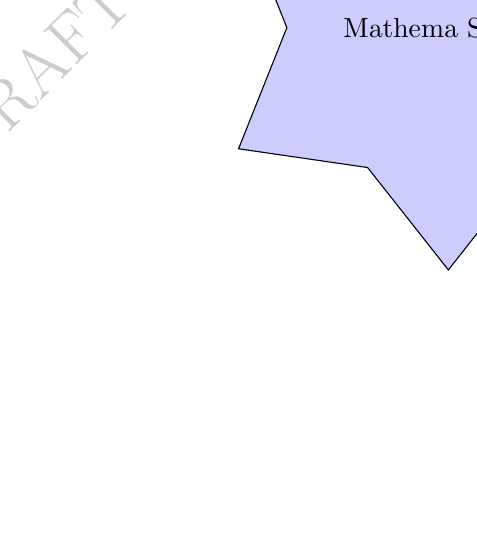
\begin{tikzpicture}
		\tikz \node [fill=blue!20,star,star points=6,draw] {Mathema Shukur };
	\end{tikzpicture}
	\\
	যাদের জন্যে প্রযোজ্যঃ  	\textcolor{magenta}{একাদশ ও দ্বাদশ শ্রেণীর শিক্ষার্থী} \\
	বিষয়ঃ \textcolor{magenta}{উচ্চতর গণিত ১ম পত্র} \\
	অধ্যায়ঃ \textcolor{magenta}{৩-সরলরেখা}\\ 
	Subtopicঃ  \textcolor{magenta}{  মূলবিন্দু ধারণকারী কোণের সমদ্বিখণ্ডক সমীকরণ নির্ণয় Bisector of the Angle which Contains the Origin}\\
	\\
	\textcolor{blue}{$a_1x+b_1y+c_1=0$ এবং $a_2x+b_2y+c_2=0$ রেখাদ্বয়ের অন্তর্ভুক্ত  কোণের সমদ্বিখণ্ডকের সমীকরণ \\
		\\
		$\frac{a_1x+b_1y+c_1}{\sqrt{a_1^2+b_1^2}}=\pm \frac{a_2x+b_2y+c_2}{\sqrt{a_2^2+b_2^2}}$}\\
	\\
	\begin{tabular}{|c|c|}
		\hline 
		শর্ত	& মূলবিন্দু ধারণকারী কোণের সমদ্বিখণ্ডক  \\ 
		\hline  
		$c_1\,c_2>0$	& $\frac{a_1x+b_1y+c_1}{\sqrt{a_1^2+b_1^2}}=\textcolor{red}{+} \frac{a_2x+b_2y+c_2}{\sqrt{a_2^2+b_2^2}}$\\
		\hline 
		$c_1\,c_2<0$	& $\frac{a_1x+b_1y+c_1}{\sqrt{a_1^2+b_1^2}}=\textcolor{red}{-} \frac{a_2x+b_2y+c_2}{\sqrt{a_2^2+b_2^2}}$\\
		\hline 
	\end{tabular}\\
	\\ 
\\
\\
	$3x+2y-6=0$ এবং $2x+3y-8=0$ রেখাদ্বয়ের অন্তর্গত  মূলবিন্দু ধারণকারী কোণের সমদ্বিখণ্ডকের সমীকরণ নির্ণয় কর  \\
\\
$c_1=-6,\quad c_2=-8$\\
\\
$c_1\,\,c_2=(-6)(-8)=48$\\
\\
$c_1\,\,c_2>0$\\ 
\\
	\begin{align*}
		\frac{a_1x+b_1y+c_1}{\sqrt{a_1^2+b_1^2}}&=\textcolor{red}{+} \frac{a_2x+b_2y+c_2}{\sqrt{a_2^2+b_2^2}}\\
		\\
		\frac{3x+2y-6}{\sqrt{(3)^2+(2)^2}}&=\textcolor{red}{+} \frac{2x+3y-8}{\sqrt{(2)^2+(3)^2}}\\
		\\
		\frac{3x+2y-6}{\sqrt{13}}&=\textcolor{red}{+} \frac{2x+3y-8}{\sqrt{13}}\\
		\\
	3x+2y-6&=2x+3y-8\\
		\\
		x-y+2&=0\\
	\end{align*}
	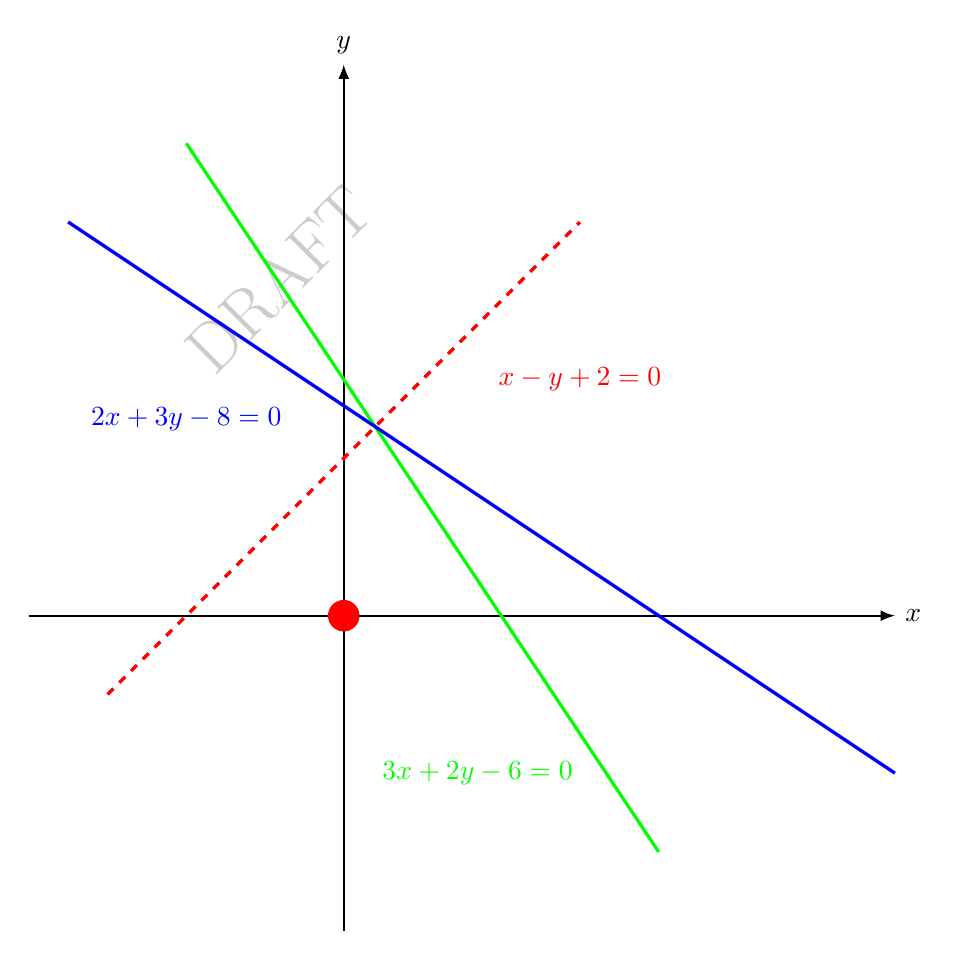
\begin{tikzpicture}[transform shape,scale=1]
		\draw [-latex,thick](-4,0) -- (7,0) node[right] {$x$} coordinate(x axis);
		\draw [-latex,thick](0,-4) -- (0,7) node[above] {$y$} coordinate(y axis);
		\fill[red] (0,0) circle (2 mm);
		\node at (1.7,-2) {$\textcolor{green}{3x+2y-6=0}$};		
		\node at (3,3) {$\textcolor{red}{x-y+2=0}$};	
		\node at (-2,2.5) {$\textcolor{blue}{2x+3y-8=0}$};	
		\draw[very thick,green] (-2,6)--(4,-3);	
		\draw[very thick,blue] (-3.5,5)--(7,-2);	
		\draw[very thick,red,dashed] (-3,-1)--(3,5);		
	\end{tikzpicture}
\\
\\
\\
$3x-4y+12=0$ এবং $8x+15y-12=0$ রেখাদ্বয়ের অন্তর্গত মূলবিন্দু ধারণকারী কোণের সমদ্বিখণ্ডকের সমীকরণ নির্ণয় কর  \\
\\
\\
$c_1=+12,\quad c_2=-12$\\
\\
$c_1\,\,c_2=(+12)(-12)=-144$\\
\\
$c_1\,\,c_2<0$\\ 
\\
\begin{align*}
	\frac{a_1x+b_1y+c_1}{\sqrt{a_1^2+b_1^2}}&=\textcolor{red}{-} \frac{a_2x+b_2y+c_2}{\sqrt{a_2^2+b_2^2}}\\
	\\
	\frac{3x-4y+12}{\sqrt{(3)^2+(-4)^2}}&=\textcolor{red}{-} \frac{8x+15y-12}{\sqrt{(8)^2+(15)^2}}\\
	\\
	\frac{3x-4y+12}{\sqrt{25}}&=\textcolor{red}{-} \frac{8x+15y-12}{\sqrt{289}}\\
	\frac{3x-4y+12}{5}&=\textcolor{red}{-} \frac{8x+15y-12}{17}\\
	17(3x-4y+12)&=-5(8x+15y-12)\\
	91x+7y+144&=0
\end{align*}
\begin{tikzpicture}[transform shape,scale=1]
	\draw [-latex,thick](-8,0) -- (7,0) node[right] {$x$} coordinate(x axis);
	\draw [-latex,thick](0,-8) -- (0,6) node[above] {$y$} coordinate(y axis);
	\fill[red] (0,0) circle (2 mm);
	\node at (4,3.5) {$\textcolor{green}{3x-4y+12=0}$};		
	\node at (-3.5,-3) {$\textcolor{red}{91x+7y+144=0}$};	
	\node at (3,-2.5) {$\textcolor{blue}{8x+15y-12=0}$};	
	\draw[very thick,green] (-8,-3)--(4,6);	
	\draw[very thick,blue] (7,-2.933)--(-4,2.933);	
	\draw[very thick,red,dashed] (-1.967,5)--(-0.967,-8);		
\end{tikzpicture}
\\
\\
\\ 
$a_1x+b_1y+c_1=0$ এবং $a_2x+b_2y+c_2=0$ রেখাদ্বয়ের অন্তর্ভুক্ত $(x_1,y_1)$ বিন্দু  ধারণকারী কোণের সমদ্বিখণ্ডকের সমীকরণ \\
\\
\\

\begin{tabular}{|c|c|}
	\hline 
	শর্ত	& $(x_1,y_1)$ বিন্দু  ধারণকারী কোণের সমদ্বিখণ্ডক  \\ 
	\hline  
	$(a_1x_1+b_1y_1+c_1)(a_2x_1+b_2y_1+c_2)>0$	& $\frac{a_1x+b_1y+c_1}{\sqrt{a_1^2+b_1^2}}=\textcolor{red}{+} \frac{a_2x+b_2y+c_2}{\sqrt{a_2^2+b_2^2}}$\\
	\hline 
	$(a_1x_1+b_1y_1+c_1)(a_2x_1+b_2y_1+c_2)<0$	& $\frac{a_1x+b_1y+c_1}{\sqrt{a_1^2+b_1^2}}=\textcolor{red}{-} \frac{a_2x+b_2y+c_2}{\sqrt{a_2^2+b_2^2}}$\\
	\hline 
\end{tabular}\\
\\ 
\end{document}